\documentclass[10pt,twocolumn,a4paper]{article}

\usepackage[a4paper,top=1.7cm,bottom=1.7cm,left=1.6cm,right=1.6cm,columnsep=0.6cm]{geometry}
\usepackage[T1]{fontenc}
\usepackage{mathptmx}
\usepackage{microtype}
\usepackage{amsmath,amssymb}
\usepackage{booktabs}
\usepackage{graphicx}
\usepackage{xcolor}
\usepackage{tikz}
\usetikzlibrary{arrows.meta,positioning,calc}
\usepackage[font=small,labelfont=bf,skip=4pt]{caption}
\usepackage{titlesec}
\usepackage{enumitem}
\usepackage[hidelinks]{hyperref}

\titleformat*{\section}{\normalsize\bfseries}
\titleformat*{\subsection}{\normalsize\bfseries\itshape}
\titlespacing*{\section}{0pt}{7pt plus 2pt minus 1pt}{3pt}
\titlespacing*{\subsection}{0pt}{5pt plus 1pt minus 1pt}{2pt}
\setlist{nosep,leftmargin=*}
\setlength{\textfloatsep}{8pt plus 2pt minus 2pt}
\setlength{\abovedisplayskip}{4pt plus 1pt minus 1pt}
\setlength{\belowdisplayskip}{4pt plus 1pt minus 1pt}

\definecolor{learn}{HTML}{2A78D6}
\definecolor{frozen}{HTML}{898781}
\newcommand{\para}[1]{\textbf{#1}\hspace{0.4em}}

\begin{document}

\twocolumn[
\begin{center}
  {\Large\bfseries ProtoCoCoOp: Knowledge Distillation and Visual Prototypes\\[2pt]
  for Base-to-Novel Generalization of CLIP\par}
  \vspace{8pt}
  {\normalsize Andrea Giampietro \qquad Marco Gandolfi \qquad Stefano Camposilvan\par}
  \vspace{2pt}
  {\small University of Trento \,·\, Deep Learning course project, a.y.\ 2024/25\par}
  {\small\url{https://github.com/giampyhatesyou/CLIP_Proto-CoCoOp}\par}
  \vspace{8pt}
  \begin{minipage}{0.86\textwidth}
  \small\noindent\textbf{Abstract.}
  Prompt learning adapts CLIP to a new task from a handful of labeled images, but the
  learned prompts overfit the classes seen in training and erode the zero-shot transfer
  that made CLIP useful in the first place. We study this base-to-novel trade-off on
  Flowers102 with 10 shots per class and propose ProtoCoCoOp, which adds two light
  components to CoCoOp: during training, a distillation term keeps the adapted model close
  to the frozen CLIP teacher; at inference, a training-free prototype residual adds visual
  evidence to the logits of the classes seen in training. With a frozen ViT-B/16 backbone
  and 37K trainable parameters, ProtoCoCoOp reaches a harmonic mean of 84.44\%, against
  74.62\% for zero-shot CLIP and 83.38\% for CoCoOp. The ablation shows why: distillation
  moves accuracy from base to novel classes, and prototypes give the base accuracy back
  without touching novel predictions.
  \end{minipage}
  \vspace{12pt}
\end{center}
]

\section{Introduction}

Vision--language models such as CLIP~\cite{clip} embed images and text in a shared space
and can recognize arbitrary categories by comparing an image with prompts such as
``a photo of a \{class\}''. When a few labeled examples of the target task are available,
prompt learning methods such as CoOp~\cite{coop} replace the hand-written prompt with
learned context vectors and improve accuracy substantially. The price is generalization:
prompts optimized on a set of \emph{base} classes transfer poorly to \emph{novel} classes
of the same task that were never seen in training~\cite{cocoop}. CoCoOp~\cite{cocoop}
reduces the problem by conditioning the prompt on each image, but a gap remains.

This report studies the base-to-novel setting on Flowers102~\cite{flowers} and asks
whether the two sides of the trade-off can be handled separately. ProtoCoCoOp
(Figure~\ref{fig:method}) keeps CoCoOp as the backbone and adds:
\begin{itemize}
  \item a \textbf{knowledge-distillation} term~\cite{kd} that pulls the student towards
        the zero-shot predictions of the frozen CLIP teacher during training, protecting
        novel-class accuracy;
  \item a \textbf{prototype residual} applied only at inference, which adds the
        similarity between the test image and per-class visual
        prototypes~\cite{protonets,tipadapter} to the logits of base classes, recovering
        the base accuracy that distillation gives up.
\end{itemize}
Neither component adds trainable parameters, and the residual needs no training at all.
Among the configurations we compare, the combination obtains the best harmonic mean
between base and novel accuracy (Table~\ref{tab:results}).

\section{Method}

\begin{figure}[t]
\centering
\resizebox{\columnwidth}{!}{%
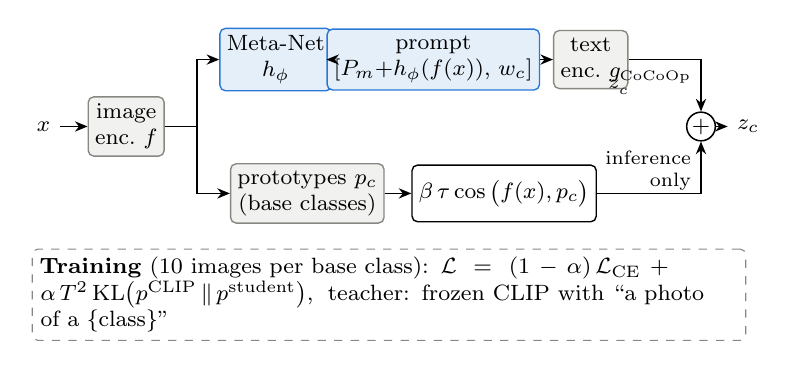
\begin{tikzpicture}[font=\footnotesize,
  box/.style={draw, rounded corners=2pt, align=center, inner sep=2.5pt, minimum height=0.72cm, line width=0.5pt},
  frz/.style={box, draw=frozen, fill=frozen!12},
  lrn/.style={box, draw=learn, fill=learn!12},
  arr/.style={-{Stealth[length=1.6mm,width=1.3mm]}, line width=0.55pt}]
  \node (img) at (0,0) {$x$};
  \node[frz] (ienc) at (1.05,0) {image\\enc.\ $f$};
  \coordinate (split) at (1.95,0);
  \node[lrn] (meta) at (2.95,0.85) {Meta-Net\\$h_\phi$};
  \node[lrn] (ctx) at (4.95,0.85) {prompt\\$[P_m{+}h_\phi(f(x)),\,w_c]$};
  \node[frz] (tenc) at (6.95,0.85) {text\\enc.\ $g$};
  \node[frz] (proto) at (3.35,-0.85) {prototypes $p_c$\\(base classes)};
  \node[box] (sim) at (5.85,-0.85) {$\beta\,\tau\cos\big(f(x),p_c\big)$};
  \node[circle, draw, inner sep=0.6pt, line width=0.55pt] (sum) at (8.35,0) {$+$};
  \node (out) at (8.95,0) {$z_c$};
  \draw[arr] (img) -- (ienc);
  \draw[line width=0.55pt] (ienc) -- (split);
  \draw[arr] (split) |- (meta);
  \draw[arr] (split) |- (proto);
  \draw[arr] (meta) -- (ctx);
  \draw[arr] (ctx) -- (tenc);
  \draw[arr] (proto) -- (sim);
  \draw[arr] (tenc.east) -| node[pos=0.72, left, font=\scriptsize] {$z^{\mathrm{CoCoOp}}_c$} (sum.north);
  \draw[arr] (sim.east) -| node[pos=0.72, left, font=\scriptsize, align=right] {inference\\only} (sum.south);
  \draw[arr] (sum) -- (out);
  \node[draw=frozen, dashed, rounded corners=2pt, align=left, inner sep=3pt, text width=8.85cm, anchor=north west]
    at (-0.15,-1.55) {\textbf{Training} (10 images per base class):
    $\mathcal{L} = (1-\alpha)\,\mathcal{L}_{\mathrm{CE}} + \alpha\,T^2\,
    \mathrm{KL}\big(p^{\mathrm{CLIP}}\,\|\,p^{\mathrm{student}}\big)$,\;
    teacher: frozen CLIP with ``a photo of a \{class\}''};
\end{tikzpicture}}
\caption{ProtoCoCoOp. Blue blocks are trained (37K parameters), grey blocks are frozen
CLIP. Distillation acts only during training; the prototype residual only at inference
and only on base classes.}
\label{fig:method}
\end{figure}

\subsection{Prompt learning with CoCoOp}
CLIP encodes an image $x$ into $f(x)$ and a text $t$ into $g(t)$, both L2-normalized, and
scores class $c$ with the scaled cosine similarity $z_c = \tau\,\langle f(x), g(t_c)\rangle$,
where $\tau$ is CLIP's learned logit scale. CoOp~\cite{coop} replaces the words of a
hand-written prompt with $M$ learnable context vectors, $t_c = [P_1,\dots,P_M,w_c]$, where
$w_c$ is the embedding of the class name. CoCoOp~\cite{cocoop} adds a small Meta-Net
$h_\phi$ that maps the image feature to a bias shared by all context tokens,
\begin{equation}
  P_m(x) = P_m + h_\phi\big(f(x)\big), \qquad m = 1,\dots,M,
\end{equation}
so that the prompt adapts to each instance. Only $\{P_m\}$ and $\phi$ are trained, with
cross-entropy on the base classes; both encoders stay frozen.

\subsection{Distillation from the frozen teacher}
Let $z^{s}$ be the student logits and $z^{t}$ the logits of the same frozen CLIP with the
hand-written prompt ``a photo of a \{class\}''. Following Hinton et al.~\cite{kd}, we
minimize
\begin{equation}
  \mathcal{L} = (1-\alpha)\,\mathcal{L}_{\mathrm{CE}}
  + \alpha\,T^2\,\mathrm{KL}\big(\sigma(z^{t}/T)\,\|\,\sigma(z^{s}/T)\big),
\end{equation}
with $\alpha = 0.3$ and $T = 2$, where $\sigma$ is the softmax. The cross-entropy term
only sees base classes, while the KL term runs over the whole label vocabulary, so it also
constrains how the learned context treats class names that never receive a label. The
teacher acts as a soft anchor: the student may specialize only as far as it stays
consistent with CLIP's zero-shot geometry. KgCoOp~\cite{kgcoop} and
PromptSRC~\cite{promptsrc} use related regularizers towards the frozen model.

\subsection{Prototype residual at inference}
For each base class $c$ we encode its 10 training images, plus 10 augmented views of each
(random crop, horizontal flip, rotation up to $30^\circ$, color jitter), with the frozen
image encoder, and average the 110 normalized embeddings into a prototype $p_c$, normalized
again to unit length. At test time the base-class logits become
\begin{equation}
  z_c(x) = z_c^{\mathrm{CoCoOp}}(x) + \beta\,\tau\cos\big(f(x),p_c\big),
  \qquad c \in \mathcal{C}_{\mathrm{base}},
\end{equation}
with $\beta = 0.5$; novel classes have no prototype and keep their CoCoOp logits. The
residual is related to the cache model of Tip-Adapter~\cite{tipadapter}, but it uses one
mean prototype per class and is added to the prompt-based classifier instead of replacing
it. It costs one $512 \times 51$ matrix product per image and no gradient step.

\section{Experimental setup}

\para{Data and protocol.} Flowers102~\cite{flowers} contains 102 flower species. Following
the base-to-novel protocol of~\cite{cocoop}, the first 51 classes are base and the other 51
novel. We train on the 10 images per base class of the official training split (510
images), select the checkpoint on the base classes of the validation split, and test on
the official test split. Base and novel accuracy are each measured as 51-way
classification among the classes of their split, and we report their harmonic mean
$\mathrm{HM} = 2BN/(B+N)$, which rewards balanced performance.

\para{Implementation.} CLIP ViT-B/16, frozen and run in fp32. $M = 8$ context vectors
drawn from $\mathcal{N}(0, 0.02^2)$; Meta-Net $512 \to 32 \to 512$ with ReLU; 37,408
trainable parameters, about 0.025\% of CLIP. SGD with learning rate 0.002, momentum 0.9,
weight decay $5\cdot10^{-4}$, batch size 1 and a cosine schedule over at most 15 epochs,
with early stopping (patience 5) on base validation accuracy; seed 42. All configurations
share these hyper-parameters. Zero-shot CLIP uses the prompt ``a photo of a \{class\}, a
type of flower.''

\section{Results}

\begin{table}[t]
\centering
\small
\begin{tabular}{@{}lccc@{}}
\toprule
Method & Base & Novel & HM \\
\midrule
CLIP zero-shot~\cite{clip}       & 71.33          & \textbf{78.24} & 74.62 \\
CoCoOp~\cite{cocoop}             & 93.57          & 75.19          & 83.38 \\
CoCoOp + KD                      & 87.18          & 76.47          & 81.47 \\
\textbf{ProtoCoCoOp (ours)}      & \textbf{93.85} & 76.74          & \textbf{84.44} \\
\bottomrule
\end{tabular}
\caption{Test accuracy (\%) on Flowers102, base-to-novel, 10 shots per base class,
ViT-B/16. ProtoCoCoOp is CoCoOp trained with KD and evaluated with the prototype
residual.}
\label{tab:results}
\end{table}

\begin{figure}[t]
\centering
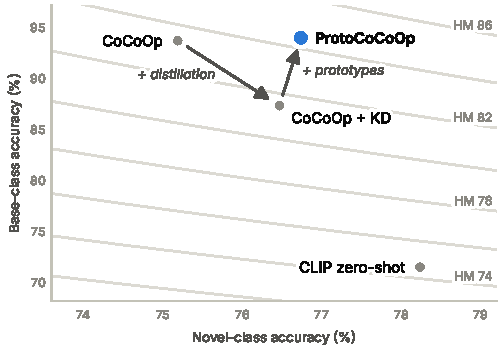
\includegraphics[width=\columnwidth]{figures/tradeoff.pdf}
\caption{Base vs.\ novel accuracy. Grey curves join points with equal harmonic mean.
Distillation moves CoCoOp down and to the right; prototypes then move it straight up.}
\label{fig:tradeoff}
\end{figure}

\para{Prompt learning buys base accuracy with novel accuracy.} CoCoOp improves base
accuracy by 22.2 points over zero-shot CLIP and loses 3.1 points on novel classes; HM still
rises to 83.38 because the base gain is much larger. Our zero-shot numbers (71.33 / 78.24)
are close to the 72.08 / 77.80 reported in~\cite{cocoop} on the same split, a useful check
of the evaluation pipeline.

\para{Distillation moves the operating point rather than improving it.} Adding KD recovers
1.3 novel points but costs 6.4 base points, so HM drops to 81.47. On its own, distillation
trades one side of the problem for the other.

\para{Prototypes give the base accuracy back.} CoCoOp + KD and ProtoCoCoOp use the same
training objective and differ only at inference, so the base gain from 87.18 to 93.85
($+6.7$) comes from the prototype residual. Prototypes cannot affect novel predictions; the
0.27-point difference in novel accuracy between the two rows is variation between their
training runs. The final model matches CoCoOp on base classes (93.85 vs.\ 93.57) while
keeping 1.55 more points on novel ones, for the best HM: 84.44, that is $+1.06$ over CoCoOp
and $+9.82$ over zero-shot CLIP.

\section{Discussion}

\para{What the experiments show.} On this benchmark the trade-off of prompt learning can
be split into two problems handled at different times: a training-time regularizer that
preserves CLIP's zero-shot behavior, and an inference-time memory that restores
specialization where labeled data exist. The two act on different sides of the
trade-off---distillation on the text side and on all classes, prototypes on the visual
side and on base classes only---which is why their effects add up in HM instead of
cancelling out.

\para{What they do not show.} The evidence is narrower than that conclusion. (i)~Every
number comes from one training run (seed 42) on one dataset; a gain of about one HM point
over CoCoOp should be confirmed over several seeds and the other datasets
of~\cite{cocoop}. (ii)~The prototype-only configuration (CoCoOp + prototypes without KD) is
supported by the code but not reported, so the ablation does not establish that
distillation is necessary in the final model. (iii)~The residual is safe only because base
and novel classes are evaluated separately; in a joint 102-way decision a positive term on
base classes alone would bias predictions towards them and would need calibration.
(iv)~Distillation sees the names of novel classes, though never their images or labels,
which is slightly weaker than a strictly inductive protocol. (v)~No sensitivity analysis
of $\alpha$, $\beta$ and $T$ is reported. Novel accuracy also stays 1.5 points below
zero-shot CLIP: the method narrows the generalization gap rather than closing it.

\section{Conclusion}

ProtoCoCoOp shows that a few-shot adapted CLIP can keep its specialization while giving up
less of its zero-shot generalization, using two components that add no trainable
parameters: distillation during training and prototype residuals at inference. Natural
next steps are a multi-seed evaluation on the eleven datasets of the CoCoOp benchmark, the
missing prototype-only ablation, a joint base-and-novel evaluation with a calibrated
residual, and a teacher restricted to base-class names and prompted with the stronger
dataset-specific template.

{\footnotesize
\begin{thebibliography}{9}
\setlength{\itemsep}{1pt}
\bibitem{clip} A.~Radford et al. Learning transferable visual models from natural language
  supervision. \emph{ICML}, 2021.
\bibitem{coop} K.~Zhou, J.~Yang, C.~C.~Loy, Z.~Liu. Learning to prompt for vision-language
  models. \emph{IJCV}, 2022.
\bibitem{cocoop} K.~Zhou, J.~Yang, C.~C.~Loy, Z.~Liu. Conditional prompt learning for
  vision-language models. \emph{CVPR}, 2022.
\bibitem{flowers} M.-E.~Nilsback, A.~Zisserman. Automated flower classification over a
  large number of classes. \emph{ICVGIP}, 2008.
\bibitem{kd} G.~Hinton, O.~Vinyals, J.~Dean. Distilling the knowledge in a neural network.
  \emph{arXiv:1503.02531}, 2015.
\bibitem{protonets} J.~Snell, K.~Swersky, R.~Zemel. Prototypical networks for few-shot
  learning. \emph{NeurIPS}, 2017.
\bibitem{tipadapter} R.~Zhang et al. Tip-Adapter: Training-free adaption of CLIP for
  few-shot classification. \emph{ECCV}, 2022.
\bibitem{kgcoop} H.~Yao, R.~Zhang, C.~Xu. Visual-language prompt tuning with
  knowledge-guided context optimization. \emph{CVPR}, 2023.
\bibitem{promptsrc} M.~U.~Khattak et al. Self-regulating prompts: Foundational model
  adaptation without forgetting. \emph{ICCV}, 2023.
\end{thebibliography}
}

\end{document}
